
\documentclass[draft,linenumbers]{agujournal2019}

\usepackage{url} 
\usepackage{lineno}
% \usepackage[inline]{trackchanges} 
\usepackage{soul}
\usepackage{natbib}
\usepackage{float}

%\draftfalse

\journalname{JGR Oceans}

%%%%%%%%%%%%%%%%%%%%%%%%%%%%%%%%%%%

%% MACROS
\newcommand{\MKE}{\overline{\textrm{KE}}}
\newcommand{\mKE}{\textrm{MKE}}
\newcommand{\KE}{\textrm{KE}}
\newcommand{\MEKE}{\overline{\textrm{EKE}}}
\newcommand{\EKE}{\textrm{EKE}}
\newcommand{\MCEKE}{\overline{\textrm{CEKE}}}
\newcommand{\CEKE}{\textrm{CEKE}}
\newcommand{\MnCEKE}{\overline{\textrm{nCEKE}}}
\newcommand{\nCEKE}{\textrm{nCEKE}}
\newcommand{\cEddy}{\textrm{cEddy}}

\begin{document}
\title{Climatology, seasonality and trends of oceanic coherent eddies}

\authors{Josu\'e Mart\'inez-Moreno\affil{1}, Andrew McC. Hogg\affil{1}, and Matthew England\affil{2}}
\affiliation{1}{Research School of Earth Science and ARC Center of Excellence for Climate Extremes, Australian National University, Canberra, Australia}
\affiliation{2}{Climate Change Research Centre (CCRC), UNSW Australia, Sydney NSW, Australia}

\correspondingauthor{Josu\'e Mart\'inez-Moreno}{josue.martinezmoreno@anu.edu.au}

\begin{keypoints}
	\item Kinetic energy of coherent eddies 
	contain around 30\% of the 
	surface ocean kinetic energy budget.
	\item Seasonal cycle of the number of coherent eddies and 
	coherent eddy amplitude reveal a 3-6 month lag to wind forcing
	\item The coherent eddy amplitude has increase at 
	a rate of 3 cm per decade since 1993.
\end{keypoints}


\begin{abstract}
	
	Ocean eddies influence regional and global climate through mixing and transport of heat and properties. 
	One of the most recognizable and ubiquitous feature of oceanic eddies are vortices with spatial scales of tens to hundreds of kilometers, frequently referred as ``mesoscale eddies" or ``coherent eddies". 
	Coherent eddies are known to transport properties across the ocean and to locally affect near-surface wind, cloud properties and rainfall patterns. Although coherent eddies are ubiquitous, yet their climatology, seasonality and long-term temporal evolution remains poorly understood. 
	Thus, we examine the kinetic energy contained by coherent eddies and we present the annual, interannual, and long-term changes of automatically identified coherent eddies from satellite observations and a state of the art numerical simulation from 1993 to 2018. 
	Satellite observations show that around 40\% of the kinetic energy contained by ocean eddies corresponds to coherent eddies. 
	Additionally, a strong hemispherical seasonal cycle is observed, on top of a 3--6 months lag between the wind forcing and the response of the coherent eddy field. 
	Furthermore, the seasonality of the number of coherent eddies and their amplitude reveals that the number of coherent eddies responds faster to the forcing ($\sim$3 months), while the coherent eddy amplitude is lagged by $\sim$6 months.  
	There are regions that show a pronounced influence of coherent eddies, notably, the East Indian Ocean, the East Tropical Pacific Ocean, and the South Atlantic Ocean. 
	In these locations, a strong seasonal cycle and interannual variability can be observed in both satellite and numerical models. Although, there is agreement between these products on the seasonality of the number of eddies, the seasonality of the coherent eddy amplitude between these products show some inconsistencies. 
	Long-term trends of the coherent eddy amplitude from satellite observations and the state of the art model show significant increases in the eddy amplitude of $\sim$3cm per decade in large portions of the ocean, while the number of coherent eddies remains constant. 
	Our analysis highlight the relative importance of the coherent eddy fiend in the ocean kinetic energy budget, imply a strong response of the eddy number and eddy amplitude to the surface wind at different time-scales, and showcases for the first time seasonality, and multidecadal trends of the coherent eddy properties. 

	\noindent\textbf{Plain language summary}
	
\end{abstract}	

% -	Ratios of KE!! 
% -	Coherent signature + seasonality  and non-coherent signature (not key point)
% -	Identify regions dominated by coherent eddies
	
\section{Introduction}

Mesoscale ocean variability with spatial scales of tens to hundreds of kilometers is comprised by processes such as vortices, waves, and jets \citep{Ferrari_energy_2009, Fu_Eddy_2010}. 
These mesoscale processes are highly energetic, and they play a crucial role in the transport of heat, salt, momentum and other tracers through the ocean \citep{Wunsch_energetics_2004, Wyrtki_Eddy_1976, Gill_Energy_1974}. Possibly, the most recognizable and abundant process observed from satellites are mesoscale vortices. Although mesoscale vortices are commonly refer in literature as ``mesoscale eddies", this term is also often used to describe mesoscale ocean variability (time-varying component of flow), thus, here we will refer to mesoscale vortices as coherent eddies. 


Coherent eddies are circular currents and according to their rotational direction, the sea surface height anomaly within a coherent eddy can have a negative or positive sea surface height anomaly (cold core and warm core coherent eddies, respectively). 
This characteristic sea surface height signature of coherent eddies has been utilized to automatically identified and tracked coherent eddies from satellite altimetry \citep{Cui_eddy_identification_2020,Martinez_Kinetic_2019, Ashkezari_eddies_2016, Faghmous_A_2015,Chelton_Global_2007}. 
Automated identification algorithms of coherent eddies have shown their ubiquity in the oceans, with a predominant influence at hotpots of eddy activity such as boundary currents and the Antarctic Circumpolar current. In these regions, \citet{Chelton_The_2011} estimated that coherent eddies contribute around 40--50\% of the mesoscale kinetic energy \citep{Chelton_The_2011} and thus a significant fraction of the total kinetic energy \citep{Ferrari_energy_2009}. Although this unique estimate showcases the importance of the mesoscale coherent eddy field, the energy contained by coherent eddies was estimated by extracting the the geostrophic velocities within the detected coherent eddies, thus it is possible it may contain energy from other processes. Coherent eddies are not only abundant and may have a large proportion of the surface kinetic energy budget, but they also are essential in the ocean dynamics as concluded by many previous studies \citep{Patel_SO_eddies_2020,Schubert_submesoscale_2019,Pilo_eddy_2015,Frenger_Southern_2015,Frenger_Imprint_2013,BeronVera_Agulhas_2013,Siegel_Bio_2011,Hogg_Interdecadal_2006}.


There is broad consensus that mesoscale eddy kinetic energy has a pronounced seasonal variability \citep{Uchida_Seasonality_2017,Kang_On_2017,Qiu_seasonal_2004, Qiu_seasonal_1999}, several hypothesis proposed to explain this include: seasonal variations of atmospheric forcing \citep{Sasaki_seasonal_2014}, seasonality of the mixed layer depth \citep{Qiu_seasonal_2014,Callies_season_2015}, seasonality in the intensity of barotropic instability \citep{Qiu_seasonal_2004}, variability of the baroclinic instability due to seasonality of the vertical shear \citep{Qiu_seasonal_1999}, and a seasonal lag of the inverse energy cascade (energy is transported between scales from small to large; \citealp{Arbic_cascade_2013}) in combination with the presence of a front in the mixed layer, which can lead to a seasonal cycle of the baroclinic instability \citep{Qiu_seasonal_2014}. 
All  these factors are likely to influence the seasonal cycle of coherent eddies, however the seasonality of the coherent component of the eddy kinetic energy, as well as the seasonal cycle of the coherent eddy statistics remains unknown.

% Front in ML, then frontal baroclinic instability
% Vertical Shear = Interior baroclinic instability.

On one hand, processes such as barotropic and baroclinic instabilities could control the seasonality of coherent eddies in the ocean. 
On the other hand, recent studies using observations and eddy-permitting climate models suggest several long term adjustments of the global ocean capable of longterm changes in the coherent eddy field. 
Such readjustments include a multidecadal increase in the ocean stratification resulted from temperature and salinity changes \citep{Li_stratification_2020}, a horizontal readjusment of the sea surface temperature gradients \citep{Ruela_SST_trends_2020,Bouali_SST_grad_trends_2017,Cane_SST_trends_1997}, and an intensification of the kinetic energy, eddy kinetic energy, and mesoscale eddy kinetic energy over the last 3 decades as a consequence of an increase in wind forcing \citep{Hu_acceleration_2020,Wunsch_speeding_2020,Martinez_Kinetic_2021}. 
These readjustment are directly tight with the generation of coherent eddies, thus they could modify the long term response of the mesoscale coherent eddy field. 

\textcolor{purple}{\scriptsize \textbf{Andy suggested to move the previous paragraph somewhere else, but I don't know where would it fit best, I think it will be confusing to introduce long-term trends before the seasonal cycle. Any suggestion? Perhaps merge both paragraphs?} i.e. $\dots$ of the baroclinic instability \citep{Qiu_seasonal_2014}. On one hand, processes such as barotropic and baroclinic instabilities could control the seasonality of coherent eddies in the ocean.  On the other hand, recent studies $\dots$ All these seasonal factors and longterm readjusments directly influence the annual and decadal response of the coherent eddy field, however the seasonality of the coherent component of the eddy kinetic energy, as well as the seasonal cycle and trends of the coherent eddy statistics remain unknown. \textbf{What do you think?}}

Here we present a new estimate and climatology of the coherent eddy kinetic energy by reconstructing the coherent eddy signature from satellite observations, the seasonal cycle of the coherent eddy kinetic energy and seasonal cycle and longterm trends of the coherent eddy properties over the satellite record. 
Moreover, we investigate regions where coherent eddies dominate the eddy kinetic energy field. 
This paper is structured as follows:  the data sources and methodology are described in section \ref{sec:Methods}.
Then, we present the climatology, energy ratios and global seasonality of the coherent eddy kinetic energy in subsection \ref{subsec:CEKE_climatology}. 
Subsection \ref{subsec:CE_stats} presents the global climatology and seasonality of coherent eddy properties, followed by the seasonal cycle and coherent eddy property time-series in regions dominated by coherent eddies (subsection \ref{subsec:CE_regional_stats}). 
We then focus our attention to the longterm changes of the coherent eddy properties (section \ref{sec:CE_trends}). 
Finally, section \ref{sec:Conclusions} summarizes the main results and discuss the implications of this study.

\section{Methods}
\label{sec:Methods}
% %	
% %	We compute global climatological montly KE, EKE, TEKE and TRKE by processing satellite observations and implementing TrackEddy an coherent eddy identification-reconstruction algorithm, with the capability to separate the Kinetic Energy from coherent and non-coherent features. The present study expands our understanding in the seasonal cycle, inter-annual variability and decadal trends.
% %	
% %	
	\subsection{Data}
	

	\subsection{Coherent eddy identification algorithm}


	\subsection{Kinetic Energy decomposition}

	Kinetic energy is commonly divided into the mean and time-varying components through a Reynolds decomposition. At a given time, the velocity field $\mathbf{u} = (u,v)$ is split into the time mean ($\mathbf{\overline{u}}$) and time varying components ($\mathbf{u'}$). Additionally, we further decompose the eddy kinetic energy into the eddy kinetic energy contained by coherent features ($\mathbf{u'_e}$) and non-coherent ($\mathbf{u'_n}$). Therefore the KE equation can be written as:
	
	\begin{equation}
		\mathrm{KE} = \underbrace{\overline{u}^2 + \overline{v}^2}_{\mKE} + 
		\underbrace{\underbrace{{u'}_e^2+{v'}_e^2}_{\CEKE}  + \underbrace{{u'}_n^2+{v'}_n^2}_{\nCEKE} + \mathcal{O}_c^2 }_{\EKE} + \mathcal{O}^2
	\end{equation}
	% \underbrace{ u'_e^2 + v'_e^2 }_{CEKE} + \underbrace{ u'_n^2 + v'_n}^2}_{nCEKE} 
	% + \mathcal{O}^2}_{\mathbf{u'}^2} + \mathbf{\overline{u}}\mathbf{u'}
	Due to the properties of this decomposition, the second order term $\mathcal{O}^2$ is zero when averaged over the same period as $\mathbf{\overline{u}}$. However, $\mathcal{O}_c^2$ is only negligible when averaged in time and space. For more information about the decomposition of the field into coherent features and non-coherent features refer to \citet{Martinez_Kinetic_2019}. A global snapshot of each component of kinetic energy decomposition is shown in figure \ref{fig:eddy_snapshot}, where the imprint of the coherent eddies corresponds to rings of kinetic energy.

	\begin{figure}
	    \centering
	    \includegraphics[width=1\textwidth]{figures/snapshot_ke_maps_satellite.pdf}
	    \caption{Snapshot of surface kinetic energy ($\MKE$), surface eddy kinetic energy ($\MEKE$), surface coherent eddy kinetic energy ($\MCEKE$), and surface non-coherent eddy kinetic energy ($\MnCEKE$) for the 1st of January 2017.}
	    \label{fig:eddy_snapshot}
	\end{figure}


% %	
% %	Qualitatively KE seasonality is similar to TKE and therefore we will focus mostly on the seasonality of TKE.

	\section{Results}
	\label{sec:Results}
	
	\subsection{Coherent Eddy Energetics}
	\label{subsec:CEKE_climatology}

	\textbf{Figure 2}
	\begin{itemize}
		\item All KE components have large energy contents in the boundary currents and antarctic circumpolar current. 
		\item In many cases is the same, but there actually some differences There are several regions where the coherent component is larger than the non-coherent, we will investigate these in more detail in section XX.
	\end{itemize}

	\begin{figure}
	    \centering
	    \includegraphics[width=1\textwidth]{figures/mean_ke_maps_satellite.pdf}
	    \caption{Climatology of surface kinetic energy ($\MKE$), surface eddy kinetic energy ($\MEKE$), surface coherent eddy kinetic energy ($\MCEKE$), and surface non-coherent eddy kinetic energy ($\MnCEKE$) between 1993-2018.}
	    \label{fig:eddy_climatology}
	\end{figure}

	% mean surface eddy kinetic energy (EKE)
	% 364 and surface eddy kinetic energy trend between 1993-2020 (a) Zonally averaged SSH
	% 365 trend; (b) map of SSH trend (92.1% of area is statistically significant above the 95% con-
	% 366 fidence level; for spatial distribution refer to Extended Data Fig. 1a); (c) zonally averaged
	% 367 mean EKE; (d) map of mean EKE; (e) zonally averaged EKE trend; (f) map of EKE trend
	% 368 (55.4% of area is statistically significant above the 95% confidence level; see Extended
	% 369 Data Fig. 1b).

	\textbf{Figure 3}
	\begin{itemize}
		\item $\MEKE$ is responsible of almost all the $\MKE$ across the ocean, except for regions with persistent currents over time, such as the mean boundary current locations, equatorial pacific currents and regions in the Antarctic Circumpolar current, where the EKE explains around 40\% of the $\MKE$
		\item This estimate is consistent with that of Chelton.
		\item $\MEKE$ Explains $~80\%$ of $\MKE$, while $\MCEKE$ is $~45\%$ of $\MEKE$ and $\MnCEKE$  is $~60\%$ of $\MEKE$ 
		\item $\MCEKE$ is large equatorwards from the Kuroshio current and Agulhas current.
		\item Areas with the largest coherent contribution are located in the South of Australia $\MCEKE$ and South Atlantic
		\item 
		\item $\MnCEKE$ has a large amount of energy at high latitudes, this could be a consequence of the satellites not resolving the mesoscale coherent eddies. 
		\item Global averages of the ratios show $\MEKE$ explains around 78\% of the ocean $MKE$ field, while coherent eddies and non coherent eddy features contain 49\% and 59\% per decade. Note this values don't add to 1 as there are cross terms that contain around XX\% of the total energy.
	\end{itemize}


	\begin{figure}
	    \centering
	    \includegraphics[width=1\textwidth]{figures/eke_ratio_map_easy.pdf}
	    \caption{Ratios of the kinetic energy components. a) Map of the proportion of mean eddy kinetic energy ($\EKE$) versus mean kinetic energy ($\MKE$);
		b) Map of the percentage of mean coherent eddy kinetic energy ($\MCEKE$) versus mean eddy kinetic energy ($\MEKE$);
		c) Map of the percentage of mean non-coherent eddy kinetic energy ($\MnCEKE$) versus mean eddy kinetic energy ($\MEKE$);
		d) Global averaged percentage of mean eddy kinetic energy ($\left<\MEKE\right>$) versus the global mean kinetic energy ($\left<\MKE\right>$), and percentage of mean coherent eddy kinetic energy ($\left<\MCEKE\right>$) and mean non coherent eddy kinetic energy ($\left<\MnCEKE\right>$) versus global mean eddy kinetic energy ($\left<\MEKE\right>$).
		}
	    \label{fig:eddy_ratio}
	\end{figure}

	\subsubsection{Seasonality}

	\textbf{Figure 4}
	\begin{itemize}
		\item The hemisphere seasonality show the  $\EKE$ and $\CEKE$ peak in summer.
		\item Response of the $\EKE$ and $\CEKE$ show a seasonal lag of $\sim$6 months to the forcing of the Winds. Make sure to note the maximum over the hemisphere, locally, the winds may peak in different months. 
		\item Methods, explain more about winds or here. 
		\item The coherent eddy field show a large interannual variability.
		\item In the Southern Ocean we observe a concentric growth as time passes, which support the increasing trends in the Southern Ocean observed by \citep{Hogg_Recent_2015,Martinez_Kinetic_2019,Martinez_Kinetic_2021}
		\item Point that in the northern hemisphere in winter the CEKE appears to be decreasing.
	\end{itemize}

	\begin{figure}
	    \centering
	    \includegraphics[width=1\textwidth]{figures/All_polar_plots.pdf}
	    \caption{Hemispherical seasonality of eddy kinetic energy ($\EKE$), coherent eddy kinetic energy ($\CEKE$). Panels a, and b show the northern hemisphere seasonal cycle, while panels c, and d correspond to the southern hemisphere. Dashed lines correspond to the seasonal cycle of the fields and dotted lines show the seasonal cycle of the wind magnitude smoothed over 120 days (moving average). The green and magenta stars show the maximum of the seasonal cycle for the kinetic energy components and the wind magnitude, respectively. The line colors show the year.}
	    \label{fig:eddy_energy_polar}
	\end{figure}
	
	\subsection{Coherent Eddy Statistics}
	\label{subsec:CE_stats}

	\textbf{Figure 5}
	\begin{itemize}
		\item A comparison with previous identified numbers show a consistent pattern in the eddy count. The difference in the magnitude could be a consequence of \citet{Chelton_Global_2007} filtering the coherent eddies with lifespans longer than 16 weeks. 
		\item Both datasets show a large number of eddies in the East North Pacific, East North Atlantic, as well as the East South Pacific, East South Atlantic and East Indian Ocean. 
		\item While the number of eddies detected in the tropics is quite small.
		\item Furthermore, there are hotspots of numbers of eddies in other regions of the ocean, such as boundary currents and the Antarctic Circumpolar Current. 
		\item An interesting feature shown in both datasets is a predominant patchiness where the count of the eddies is much larger. These puzzling pattern remains unknown. Although it looks like a propagation pattern, it could be that eddies persist for longer in those areas.
		\item The eddy amplitude as expected is maximum at the boundary currents and hotspots in the southern ocean.
		\item Interior of the gyres we can observe that there is and important amplitude of the coherent eddy field. 
		\item Preferred eddy amplitude sign in boundary currents; positive amplitude polewards to the boundary current mean location, and negative amplitude equatorwards. This is consistent with the shed of coherent eddies from the boundary currents.
		\item There regions with large $\CEKE$ ratio show also a large coherent eddy amplitude.
	\end{itemize}

	\begin{figure}
	    \centering
	    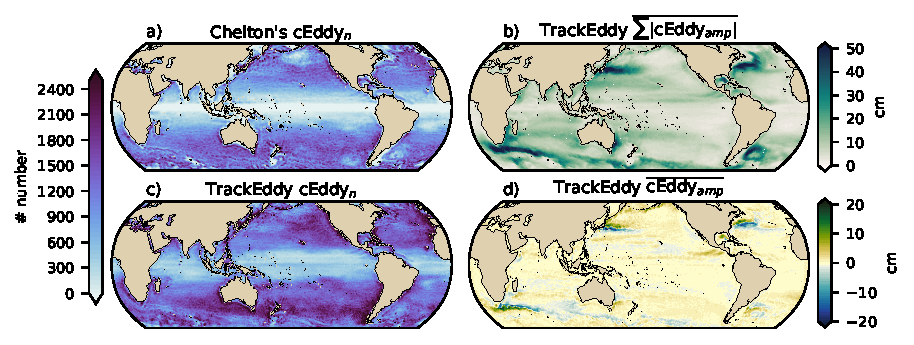
\includegraphics[width=1\textwidth]{figures/global_stats_polarity.pdf}
	    \caption{Climatology of the coherent eddy statistics. a) Climatology of the number of coherent eddies ($\cEddy_n$) identified by \citet{Chelton_Global_2007}; b) Climatology of the warm core coherent eddy amplitude ($\cEddy_{amp}$). c) Climatology of the number of coherent eddies ($\cEddy_n$) identified by \citet{Martinez_Kinetic_2019}; d) Climatology of the cold core coherent eddy amplitude ($\cEddy_{amp}$).}
	    \label{fig:eddy_stats_climatology}
	\end{figure}


	\subsubsection{Seasonality}

	\textbf{Figure 6}
	\begin{itemize}
		\item Seasonality of the number of eddies in the Northern Hemisphere peaks on May, while the Southern Hemisphere peaks on October. 
		\item The seasonality of the amplitude of the eddies is consistent with those of the Coherent eddy kinetic energy. 
		\item Interestingly, there is a 3 month lag to between the winds and the seasonality of the number of eddies, while the eddy amplitude responds approximately 6 months after the maximum winds. 
		\item Note that both coherent eddy amplitudes seem to peak around the same time. 
		\item If we look closely, the growing-shrinking concentric circles correspond to an increasing-decreasing trend. These are particularly obvious as a decrease in the eddy number in the Southern Hemisphere, and a increase in the eddy amplitude. 
	\end{itemize}

	\begin{figure}
	    \centering
	    \includegraphics[width=1\textwidth]{figures/All_polar_plots_eddy_stats_polarity.pdf}
	    \caption{Hemispherical seasonality of the coherent eddy statistics;
		a,e) seasonal cycle of the number of coherent eddies ($\cEddy_n$); b,f) seasonal cycle of the mean coherent eddy amplitude ($\cEddy_{amp}$); c,g) seasonal cycle of the warm core coherent eddies amplitude (positive $\cEddy_{amp}$); d,h) seasonal cycle of the cold core coherent eddies amplitude (negative $\cEddy_{amp}$). Panels a,b and c show the northern hemisphere seasonal cycle, while panels d,e, and f correspond to the southern hemisphere. Dashed lines correspond to the seasonal cycle of the fields and dotted lines show the seasonal cycle of the wind magnitude smoothed over 120 days (moving average). The green and magenta stars show the maximum of the seasonal cycle for each field and the wind magnitude, respectively. The line colors show the year.}
	    \label{fig:eddy_stats_polar}
	\end{figure}


	\subsection{Regional}
	\label{subsec:CE_regional_stats}
	
	% \begin{figure}
	%     \centering
	%     \includegraphics[width=1\textwidth]{figures/regional_eke_ceke_stats_no_stats.pdf}
	%     \caption{Climatology of regional statistics of the eddy field and coherent eddy field for the East Indian Ocean, East Tropical Pacific Ocean and South Atlantic Ocean. a-c) Ratio of coherent eddy kinetic energy $\CEKE$ versus eddy kinetic energy $\EKE$; d-f)  mean eddy kinetic energy ($\MEKE$); g-i) mean coherent eddy kinetic energy ($\MCEKE$).}
	%     \label{fig:regional_energy_ratios}
	% \end{figure}

	\textbf{Figure 7}
	\begin{itemize}
		\item South of the Leeuwin Current there is an important dominance fo the coherent eddy field, where it explains around 80\% of the eddy kinetic energy.
		\item Although this region does not have a large $\EKE$, we can observe a considerable amount of eddies across the region, but more importantly the coherent eddy amplitude is particularly large in those regions with coherent eddy dominance. 
		\item The solid lines show an decrease in the number of eddies, but an increase in the eddy amplitude. 
		\item Moreover, the coherent eddy number peaks in August.
		\item Meanwhile coherent eddies with the positive amplitude have a smaller amplitude than the negative, furthermore, the positive eddies peak in Jun and show a interannual modulation, while the negative eddies peak in October. 
		\item Research regional dynamics (Add here why we may expect this response.)
	\end{itemize}

	\begin{figure}
	    \centering
	    \includegraphics[width=1\textwidth]{figures/regional_ratios_and_stats_V3_0.pdf}
	    \caption{ Climatology of the eddy field and coherent eddy field at the Leeuwin Current. a) Ratio of mean coherent eddy kinetic energy ($\MCEKE$) versus mean eddy kinetic energy ($\MEKE$); b) Thick lines show the running average over 2 years and thin lines show the running average over 90 days of the coherent eddy number sum and the average absolute coherent eddy amplitude; c) Map of the number of eddies; d) Map of the average absolute coherent eddy amplitude; e) Seasonal cycle of the number of eddies f) Seasonal cycle of the positive coherent eddy amplitude. g) Seasonal cycle of the negative coherent eddy amplitude.}
	    \label{fig:leeuwin_cycle}
	\end{figure}

	\textbf{Figure 8}
	\begin{itemize}
		\item South west of the Hawai'i there is an important influence of the coherent eddies.
		\item Although, near we observe a large amount of numbers of eddies in both eddy count form Chelton and JMM, the amplitude is again responsible of the coherent eddy dominance. 
		\item Note the eddy number peaks in March, while the positive eddy amplitude peaks in October, while the negative eddies peak in June.
		\item Research regional dynamics (Add here why we may expect this response.)
	\end{itemize}

	\begin{figure}
	    \centering
	    \includegraphics[width=1\textwidth]{figures/regional_ratios_and_stats_V3_1.pdf}
	    \caption{Same as Figure \ref{fig:leeuwin_cycle} but for the Central North Pacific.}
	    \label{fig:east_tropical_cycle}
	\end{figure}

	\textbf{Figure 9}
	\begin{itemize}
		\item Here we observe that the number of eddies and eddy amplitude are large in the area where the coherent eddies dominate the eddy field.
		\item Dynamically, in this region eddies are generated due to Rossby wave propagation along the coast that becomes unstable and sheds eddies at the Tehuantepec Gulf.
		\item The seasonal cycle shows a peak in Jun, while the positive amplitude is observed in March and the negative amplitude maximum occurs in September. 
		\item Research regional dynamics (Add here why we may expect this response.)
	\end{itemize}

	\begin{figure}
	    \centering
	    \includegraphics[width=1\textwidth]{figures/regional_ratios_and_stats_V3_3.pdf}
	    \caption{Same as Figure \ref{fig:leeuwin_cycle} but for the East Tropical Pacific.}
	    \label{fig:south_atlantic_cycle}
	\end{figure}

	\textbf{Figure 10}
	\begin{itemize}
		\item Described similar to figure 7, 8, and 9
		\item Note that boundary currents have a consistent seasonal cycle in the positive and negative eddy amplitude.
		\item As expected, the seasonal cycle is opposite to BC in the northern hemisphere.
	\end{itemize}

	\begin{figure}
	    \centering
	    \includegraphics[width=1\textwidth]{figures/regional_ratios_and_stats_V3_2.pdf}
	    \caption{Same as Figure \ref{fig:leeuwin_cycle} but for the Agulhas Current.}
	    \label{fig:south_atlantic_cycle}
	\end{figure}

	\textbf{Figure 11}
	\begin{itemize}
		\item Described similar to figure 7, 8, and 9
		\item Note that boundary currents have a consistent seasonal cycle in the positive and negative eddy amplitude.
	\end{itemize}

	\begin{figure}
	    \centering
	    \includegraphics[width=1\textwidth]{figures/regional_ratios_and_stats_V3_4.pdf}
	    \caption{Same as Figure \ref{fig:leeuwin_cycle} but for the Kuroshio Current.}
	    \label{fig:south_atlantic_cycle}
	\end{figure}

	\textbf{Figure 12}
	\begin{itemize}
		\item Described similar to figure 7, 8, and 9
		\item Note that boundary currents have a consistent seasonal cycle in the positive and negative eddy amplitude.
		\item \textcolor{purple}{Delete Fig 11 or 12, they are really similar. What do you think?}
	\end{itemize}

	\begin{figure}
	    \centering
	    \includegraphics[width=1\textwidth]{figures/regional_ratios_and_stats_V3_5.pdf}
	    \caption{Same as Figure \ref{fig:leeuwin_cycle} but for the Gulf Stream.}
	    \label{fig:south_atlantic_cycle}
	\end{figure}

	\section{Trends}
	\label{sec:CE_trends}

	\textbf{Figure 13}
	\begin{itemize}
		\item The number and amplitude of coherent eddies from two eddy tracking algorithms show consistent trend patterns. 
		\item In particularly, we observe a decrease in the number of eddies in the southern ocean, as well as sectors in the North Atlantic and North Pacific. 
		\item Meanwhile the amplitude seems to be increasing in those same regions. 
		\item Some of these regions have undergone a readjustment to stronger winds, thus the observed trends in the eddy amplitude suggests an intensification of the coherent eddy field to an increase in the forcing.
		\item This increase is consistent with \citet{Martinez_Kinetic_2021}
	\end{itemize}

	\begin{figure}
	    \centering
	    \includegraphics[width=1\textwidth]{figures/all_trackeddy_trends.pdf}
	    \caption{Trends of coherent eddy statistics. a,b and c Trends of the number of identified coherent eddies from satellite observations identified using TrackEddy, satellite observations identified using Chelton's, and state of the art numerical simulation identified using TrackEddy. d,e and f Trends of the sum of the absolute value of identified coherent eddies amplitude from satellite observations identified using TrackEddy, satellite observations identified using Chelton's, and state of the art numerical simulation identified using TrackEddy. Gray stippling shows regions that are statistically significant above the 95\% confidence level.
		}
	    \label{fig:eddy_stats_trends}
	\end{figure}
	
	\section{Summary and Conclusions}	
	\label{sec:Conclusions}
	
	\acknowledgments
	
	\bibliography{biblio.bib}
	
\end{document}
